\chapter{Введение}

Задача данной методички -- дать \textbf{практические навыки} работы в консоли Linux, на примере дистрибутива Debian. В методичке обозначаются основные команды, горячие клавиши, инструменты и варианты их использования, а так же методы быстрой и эффективной работы в консоли Linux. В то же время не уходя слишком далеко в детали, оставляя некоторые инструменты и темы открытыми, чтобы читатель провёл самостоятельное их изучение, посредством чтения оригинальной документации, поиска в \href{https://google.com}{Google}, изучения \href{https://stackoverflow.com}{StackOverflow} и просмотра \href{https://youtube.com}{YouTube}. Последнее менее желательно, т.к. концентрация полезной информации в единицу времени достаточно низкая, а качество и полнота преподносимой информации желает лучшего. Никакой сайт или обучающее видео не смогут сравниться с полнотой оригинальной документации, об этом нужно всегда помнить и акцентировать внимание при изучении \textbf{абсолютно любой} технологии, программы, языка программирования, методологии и т.п.

Умение читать оригинальную документацию на английском языке (по диагонали), при этом находя то что нужно -- является критически необходимым навыком, который нужно развивать для быстрой и эффективной работы, т.к. информации на английском языке всегда было и будет больше, в силу того, что мировое сообщество его выбрало в качестве общего для общения и совместной работой между специалистами разных стран. Так же зачастую информация на английском языке является единственным источником о конфигурировании тех или иных инструментов, поэтому умение читать и понимать технические тексты на английском языке является критически важным навыком для успешной работы в IT-сфере.
\\

\noindent \textbf{P.S.} Для единообразия описания, были приняты следующие обозначения и соглашения:

\begin{itemize}
	\item \keys{ Ctrl + X } -- нажатие сочетания клавиш Ctrl+X
	\item \cmd{pwd} -- команда консоли (программа)
	\item \argum{arg} -- аругмент/параметр команды
	\item \cfgfile{/etc/passwd} -- конфигурационный файл или файл с настройками
	\item \cfgpath{/proc/} -- путь к директории с файлами процессов
\end{itemize}

\noindent  \textbf{P.S.2.} В данном методическом пособии слово \textit{команда} употребляется, как синонимом слова \textit{программа} и по сути таковой и является, если речь не идёт о встроенных командах shell-оболочек таких как: \cmd{sh}, \cmd{bash}, \cmd{zsh}.

%\section{vi}
%\section{nano}
%\section{базовые команды}
%\section{регулярные выражения}
%\section{командая строка и bash}
%\section{экранные менеджеры screen, tmux}
%\section{философия unix}
%\section{иерархия файлов}

%\begin{figure}
	%\centering
%	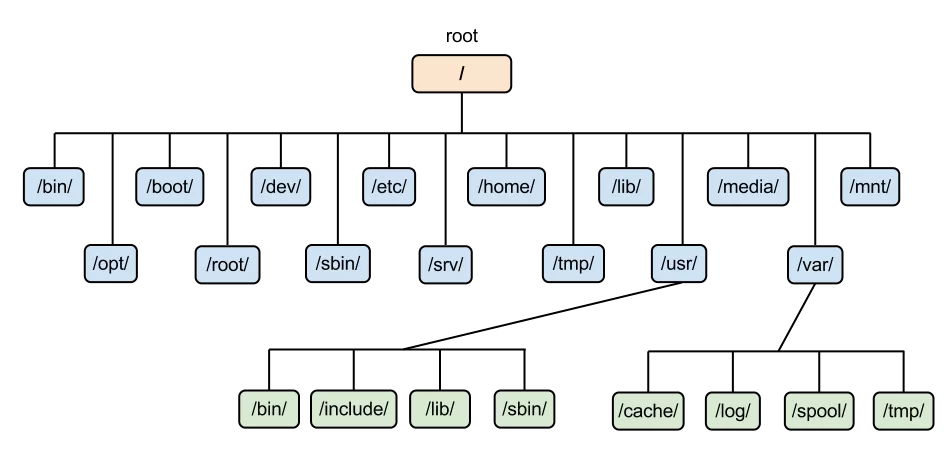
\includegraphics[width=\textwidth]{img/ch1/hfs.png}
%	\caption{Иерархия файловой системы}
%	\label{fig:galaxy}
%\end{figure}

%\keys{Сtrl + Shift + F}

%man -K IPX

%\texttt{man}

%\keys{Сtrl + Shift + F}
